% !TEX TS-program = xelatex
\documentclass[12pt]{article}
%\usepackage{amsthm,amsmath,amssymb,braket,graphicx,enumitem,booktabs,multirow,booktabs,tcolorbox,wrapfig,cancel,caption,fancyhdr,relsize,textpos,booktabs,tocbibind,titlesec}
\usepackage{amsthm,amsmath,amssymb,braket,graphicx,enumitem,booktabs,multirow,booktabs,wrapfig,cancel,caption,fancyhdr,relsize,textpos,booktabs,tocbibind,titlesec,color}
\usepackage[margin=0.5in,bottom=0.6in]{geometry}
\usepackage[T1]{fontenc}
\usepackage[hidelinks,pdfusetitle]{hyperref}
\renewcommand{\arraystretch}{1.9}
\setlength\delimitershortfall{-2pt}
\setcounter{tocdepth}{1}
\DeclareMathOperator{\sech}{sech}
\raggedbottom
\numberwithin{equation}{section}
\allowdisplaybreaks

\title{Generating Hubbard Model Solutions from Anderson Impurity Model Solutions}
\author{}%Abhirup Mukherjee, Dr. Siddhartha Lal}
\begin{document}
\maketitle
\section{Introduction}
This is an attempt to obtain various quantities like Greens functions, self-energies, spectral functions and (if possible) energies and wavefunctions of the Hubbard model, using a cluster-bath approach. The cluster-bath system is taken to be a single-impurity Anderson model with a correlated bath. The correlation will be brought about in two ways: a self-energy $\Sigma(k,\omega)$ of the bath, and a double occupancy repulsion cost $U_b$. The Hubbard and the correlated single-impurity Anderson models are defined using the Hamiltonians
\begin{align}
H_\text{hubb} &= -t^H\sum_{\sigma,\left<i,j \right>}\left(c^\dagger_{i\sigma} c_{j\sigma} + \text{h.c.}\right) + U^H\sum_i \hat n_{i \uparrow} \hat n_{i \downarrow} - \mu^H \sum_{i\sigma}\hat n_{i\sigma}\\
H_\text{siam} &= \sum_{k\sigma}\left[\epsilon_k + \Sigma(k,\omega)\right]\hat n_{k\sigma} + \epsilon_d^A \sum_\sigma\hat n_{d\sigma} + U^A \hat n_{d \uparrow} \hat n_{d \downarrow} + U_b \sum_{kk^\prime}\hat n_k \hat n_{k^\prime} - \mu^A \sum_{i\neq d,\sigma}\hat n_{i\sigma} 
	\label{hams}
\end{align}
Broadly speaking, the method involves first solving the SIAM using a unitary renormalisation group approach, to get the low energy effective theory, and then combining the low energy Hamiltonians in a symmetrized fashion to get the Hamiltonian for the Hubbard model lattice. It is reminescent of dynamical mean-field theory (DMFT) - both involve an impurity-solver that solves an auxiliary system. The difference, however, lies in the following points:
\begin{itemize}
	\item While DMFT primarily works with Greens functions and self-energies, this method involves Hamiltonians. The impurity-solver in DMFT provides an impurity Greens function (which is then equated with the local Greens function of the bath), while the impurity-solver in this method actually provides a low energy Hamiltonian.
	\item The final step of DMFT is the self-consistency equation, where the impurity and bath-local quantities are set equal. This ensures all sites, along with the impurity site, have the same self-energy, something which is required on grounds of  translational invariance. The present method, however, brings about the translational invariance in a different way. It symmetrizes the Hamiltonians itself, such that all quantites then derived from the Hamiltonian are then guaranteed to have the symmetry.
\end{itemize}
The meaning of each of these statements will become clearer when we describe the method in more detail.

\section{Philosophy of the method}
The method is closely tied to the auxiliary system approach described in \cite{martin_2016}. We can view the full Hamiltonian as a sum of two component Hamiltonians \(H_1, H_2\) connected via the interaction term \(H_{12}\).
\begin{equation}\begin{aligned}
	H = \begin{pmatrix} H_1 && H_{12} \\ H_{12}^* && H_2 \end{pmatrix} = H_1 \ket{1}\bra{1} + H_2\ket{2}\bra{2} + H_{12}\ket{1}\bra{2} + H_{12}^*\ket{2}\bra{1}
\end{aligned}\end{equation}
where \(\ket{1(2)}\) actually represents a sum over all basis kets of the subsystem 1(2). As an example, we can split the the Hubbard model Hamiltonian between a particular site \(i = p\) and the rest of the lattice as follows:
\begin{equation}\begin{aligned}
	H_\text{hubb} &= \overbrace{U^H\hat n_{p \uparrow} \hat n_{p \downarrow} - \mu^H \sum_\sigma \hat n_{p \sigma}}^{H_1} \\
		      &+ \underbrace{U^H\sum_{i \neq p}\hat n_{i \uparrow} \hat n_{p \downarrow} - \mu^H \sum_{i \neq p, \sigma} \hat n_{i \sigma} -t^H\sum_{\sigma,\left<i,j \right>\atop{i \neq p \neq j}}\left(c^\dagger_{i\sigma} c_{j\sigma} + \text{h.c.}\right)}_{H_2}\\
		      & -\underbrace{t^H\sum_{\sigma,\atop{i \in \text{N.N. of }p}}\left(c^\dagger_{i\sigma} c_{p\sigma} + \text{h.c.}\right)}_{H_{12} + H_{12}^*}\\
\end{aligned}\end{equation}
The Greens function of the full Hamiltonian can also be split in a similar fashion:
\begin{equation}\begin{aligned}
	G(\omega) = \begin{pmatrix} G_1 && G_{12} \\ G_{12}^* && G_2 \end{pmatrix} 
\end{aligned}\end{equation}
The subsystem 1 is usually taken to be the "smaller system", and consequently, subsystem 2 represents the "bath". The smaller system is typically chosen such that its eigenstates are known exactly. Progress is then made by choosing a simpler version of the bath \(H_2\) and a simpler form also for its coupling \(H_{12}\) with the smaller system. This combination of the smaller system and the simpler bath is then called the \textit{auxiliary system}. A typical auxiliary system for the Hubbard model would be the SIAM, where the impurity represents an arbitrary site \(p\) of the lattice, the bath represents the rest of the lattice sites and the hybridisation term between the impurity and the bath represents the coupling term \(H_{12}\). Such a construction is shown in fig.~\ref{cluster-bath}.
\begin{figure}[htpb!]
	\centering
	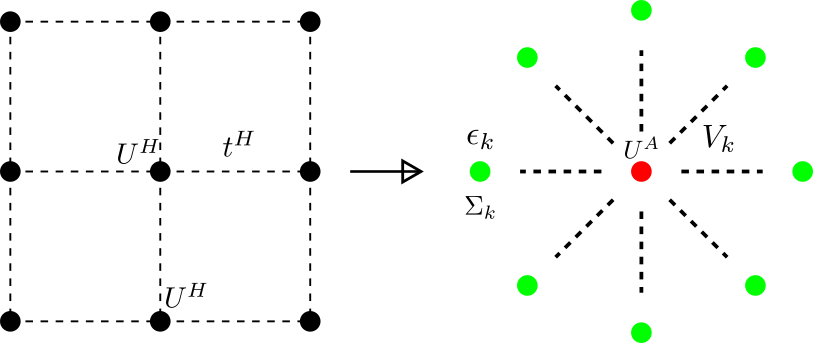
\includegraphics[width=0.8\textwidth]{./cluster-bath.png}
	\caption{\textit{Left}: Full Hubbard model lattice with onsite repulsion $U^H$ on all sites and hopping between nearest neighbour sites with strength $t^H$. \textit{Right}: Extraction of the auxiliary (cluster+bath) system from the full lattice. The central site on left becomes the impurity site (red) on the right (with an onsite repulsion $\epsilon_d$), while the rest of the $N-1$ sites on the left form a conduction bath (green circles) (with dispersion $\epsilon_k$ and correlation modelled by the self-energy $\Sigma_k(\omega)$) that hybridizes with the impurity through the coupling $V$.}
	\label{cluster-bath}
\end{figure}


The algorithm of DMFT then involves starting with some local self-energy of the bath, \(\Sigma(\omega)\), and using an impurity solver to calculate the impurity Greens function in the presence of this self-energy. This impurity Greens function is then used to calculate the impurity self-energy \(\Sigma_d(\omega)\), and the self-energy of the bath is then set equal to this impurity self-energy: \(\Sigma(\omega) = \Sigma_d(\omega)\), because we expect, on grounds of the lattice symmetry, that the impurity is the same as any other site in the bath. This is said to be the self-consistency step, because the bath self-energy is completely determined only at the end. With this updated bath self-energy, one then repeats the entire process until there is no further change in the bath self-energy at the self-consistency step.


The present method intends to calculate the quantities in a different fashion. We start with a SIAM (with a correlated bath having a non-trivial self-energy), and solve it using the unitary renormalisation group approach to get to a fixed-point Hamiltonian. The fixed point Hamiltonian will in general involve the impurity site (with renormalised parameters $\epsilon_d^*, U^*$) interacting with a smaller number of momentum states. Assuming the impurity-bath couplings are much larger than the dispersion of the bath, we can approximate the conduction bath part by a zero-mode of the kinetic energy part. What this means is that all the momentum states will then collapse to a single site (which we call the zero mode site, and represents the origin of the lattice) with a single correlation coupling $U^A_z$. Such a model, shown in fig.~\ref{and_mol} is exactly solvable. Armed with such a Hamiltonian and its spectrum, we will then create the the entire Hubbard Hamiltonian by combining the zero-mode Hamiltonians according to a prescription which is guided by the symmetries of the problem. The impurity electron will be read off as an arbitrary site, \(p\), of the lattice, while the zero-mode site becomes the site that is nearest to it. 
%TODO
\textbf{We will first demonstrate this explicitly for the Hubbard dimer. Then we will show how we can create a full Hubbard Hamiltonian by joining Anderson molecule Hamiltonians.}
\begin{figure}[htpb]
	\centering
	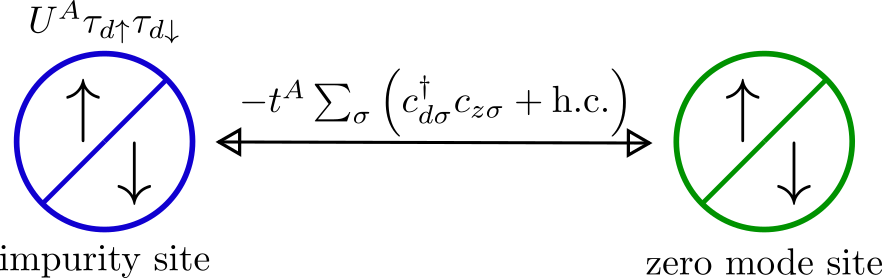
\includegraphics[width=0.6\textwidth]{./gen_siam.png}
	\caption{Correlated Anderson molecule schematic version. It consists of two sites, impurity(blue) and zero mode(green). The impurity site has onsite repulsion, and their is inter-site hopping.}
	\label{and_mol}
\end{figure}
At this point, we will assume that we have a Hubbard model in mind that has motivated a correlated SIAM as the auxiliary system, and we have performed renormalisation group analysis on this auxiliary system to get down to an effective Hamiltonian. We will also assume that the parameters of the auxiliary system have been chosen such that in the effective Hamiltonian, the impurity and zero mode have the same onsite repulsion: $U^A = U^A_z$ (this is required for translational invariance). What this all means is that the RG analysis of the bare Hubbard Hamiltonian has led to a Hubbard dimer Hamiltonian.
\begin{equation}\begin{aligned}
	H^D(U^D, t^D) \equiv -t^D\sum_\sigma\left( c^\dagger_{0\sigma}c_{1\sigma} + \text{h.c.} \right) + U^D\left( \tau_{0 \uparrow}\tau_{0 \downarrow} + \tau_{1 \uparrow}\tau_{1 \downarrow}\right)
\end{aligned}\end{equation}
This Hubbard dimer is shown in fig.~\ref{hubb-dim}.
\begin{figure}[htpb!]
	\centering
	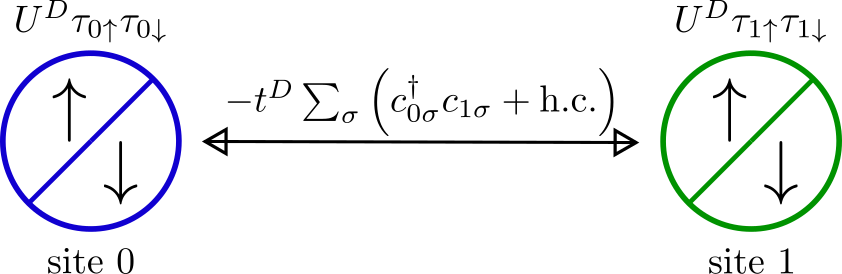
\includegraphics[width=0.6\textwidth]{./hubb_dim.png}
	\caption{Hubbard dimer schematic version. It again consists of two sites, like the Anderson molecule, but now both sites have onsite repulsion, and their is again inter-site hopping.}
	\label{hubb-dim}
\end{figure}
The next step is to combine these Hubbard dimers into a full Hubbard model, $H_\text{symm}$. Along the way, we have made two approximations:
\begin{itemize}
	\item We have replaced the full Hubbard model by an auxiliary system described by the SIAM Hamiltonian in eq.~\ref{hams}. The accuracy of this assumption is determined by the choice of the SIAM parameters, particular the self-energy and repulsion of the bath. If it is exact, then the equation
\begin{equation}\begin{aligned}
	\label{app1}
	H^H = H^A
\end{aligned}\end{equation}
holds.
	\item We then perform a unitary RG on $H^A$. This leads to a fixed-point Hamiltonian $U_A H^A U_A^\dagger$. At this point, we extract a zero mode of this Hamiltonian to obtain the Hubbard dimer Hamiltonian: $H^D = \left(U_A H^A U_A^\dagger\right)_z$, and this constitutes the second approximations we make. We tile this Hubbard dimer Hamiltonian to restore translational invariance (shown in a later section), and obtain a new Hubbard Hamiltonian, $H_\text{symm}$. If we assume that the tiling perfectly rectifies the approximation made while taking the zero mode, then we can write
\begin{equation}\begin{aligned}
	\label{app2}
	H_\text{symm} = U_A H^A U_A^\dagger
\end{aligned}\end{equation}
\end{itemize}
Combining the two eqs.~\ref{app1},\ref{app2}, we can say that
\begin{equation}\begin{aligned}
	H_\text{symm} = U_A H^H U_A^\dagger
\end{aligned}\end{equation}
which would mean that the final Hamiltonian is unitarily connected to the bare Hubbard model, but is actually made of Hubbard dimers and is hence more amenable to calculations. This of course depends on how good the approximations are and strictly speaking need to be verified.

%\section{Solution of the Hubbard dimer using the Anderson molecule}
%The Hubbard dimer and Anderson molecules (zero-mode) are defined by the following respective Hamiltonians:
%\begin{equation}\begin{aligned}
%	H^H &= -t^H\sum_{\sigma}\left(c^\dagger_{1\sigma}c_{2\sigma} + \text{h.c.}\right) + U^H\sum_{i=1,2}\hat n_{i \uparrow}\hat n_{i \downarrow} - \mu^H \sum_{\sigma, i=1,2}\hat n_{i\sigma}\\
%	H^A &= -t^A\sum_{\sigma}\left(c^\dagger_{d\sigma}c_{z\sigma} + \text{h.c.}\right) + \epsilon_d^A \sum_{\sigma}\hat n_{d\sigma} + U^A\hat n_{d \uparrow}\hat n_{d \downarrow}
%\end{aligned}\end{equation}
%In the first Hamiltonian, the indices \(i=1,2\) refer to the two lattice sites that constitute the dimer. In the second Hamiltonian, the subscript \(d\) indicates the impurity site, while the subscript \(z\) indicates the zero-mode site. First, we will assume that the Hubbard dimer is at half-filling (\(\frac{1}{2}U^H = \mu^H\)):
%\begin{equation}\begin{aligned}
%	\label{hubb_dimer}
%	H^H &= -t^H\sum_{\sigma}\left(c^\dagger_{1\sigma}c_{2\sigma} + \text{h.c.}\right) + U^H\sum_{i=1,2}\hat \tau_{i \uparrow}\hat \tau_{i \downarrow} + \left(\frac{1}{2}U^H- \mu^H\right) \sum_{\sigma, i=1,2}\hat n_{i\sigma} + \text{constant}\\
%	    &= -t^H\sum_{\sigma}\left(c^\dagger_{1\sigma}c_{2\sigma} + \text{h.c.}\right) + U^H\sum_{i=1,2}\hat \tau_{i \uparrow}\hat \tau_{i \downarrow}
%\end{aligned}\end{equation}
%Since the Hubbard Hamiltonian is at half-filling, we will also place the impurity at half-filling by setting \(\epsilon_d^A = -\frac{1}{2}U^A\):
%\begin{equation}\begin{aligned}
%	\label{and_dimer}
%	H^A &= -t^A\sum_{\sigma}\left(c^\dagger_{d\sigma}c_{z\sigma} + \text{h.c.}\right) + \left(\epsilon_d^A + \frac{1}{2}U^A\right) \sum_{\sigma}\hat \tau_{d\sigma} + U^A\hat \tau_{d \uparrow}\hat \tau_{d \downarrow} + \text{constant}\\
%	    &= -t^A\sum_{\sigma}\left(c^\dagger_{d\sigma}c_{z\sigma} + \text{h.c.}\right) + U^A\hat \tau_{d \uparrow}\hat \tau_{d \downarrow}
%\end{aligned}\end{equation}
%The first step is to recreate the Hubbard dimer Hamiltonian eq.~\ref{hubb_dimer} using the Anderson molecule Hamiltonian eq.~\ref{and_dimer}:
%\begin{equation}\begin{aligned}
%	H^H &= -t^H\sum_{\sigma}\left(c^\dagger_{1\sigma}c_{2\sigma} + \text{h.c.}\right) + U^H\sum_{i=1,2}\hat \tau_{i \uparrow}\hat \tau_{i \downarrow}\\
%	    &= \frac{1}{2}\left[-t^H\sum_{\sigma}\left(c^\dagger_{1\sigma}c_{2\sigma} + \text{h.c.}\right) + t^H\sum_{\sigma}\left(c^\dagger_{2\sigma}c_{1\sigma} + \text{h.c.}\right)\right] + \frac{1}{2} 2U^H\sum_{i=1,2}\hat \tau_{i \uparrow}\hat \tau_{i \downarrow}\\
%	    &= \frac{1}{2}\left[-t^A\sum_{\sigma}\left(c^\dagger_{d\sigma}c_{z\sigma} + \text{h.c.}\right)\bigg\vert_{z \to 2, d \to 1\atop{t^A \to t^H}} + t^A\sum_{\sigma}\left(c^\dagger_{2\sigma}c_{1\sigma} + \text{h.c.}\right)\bigg\vert_{d \to 2,z \to 1\atop{t^A \to t^H}} \right] \\
%	    &+ \frac{1}{2} \left(U^A\hat \tau_{i \uparrow}\hat \tau_{i \downarrow}\bigg\vert_{d \to 1\atop{U^A \to 2U^H}} + U^A\hat \tau_{i \uparrow}\hat \tau_{i \downarrow}\bigg\vert_{d \to 2\atop{U^A \to 2U^H}}\right)\\
%	    &=\frac{1}{2}\left[H^A\left(t^A \to t^H, U^A \to 2U^H, d \to 1, z \to 2\right) + H^A\left(t^A \to t^H, U^A \to 2U^H, d \to 2, z \to 1\right)\right]
%\end{aligned}\end{equation}
%The conclusion we can draw from this is that the Hubbard dimer Hamiltonian can be obtained from the Anderson dimer Hamiltonian in the following fashion:
%\begin{itemize}
%	\item The essential idea is that we have to create a local Hubbard Hamiltonian for each site of the Hubbard lattice by replacing the impurity label \(d\) in the Anderson dimer with the label of the particular site. So if there are two sites, we will get two local Hamiltonians obtained by replacing \(d\) with 1 and 2 respectively. For each local Hamiltonian, the zero-mode label \(z\) is replaced by the site that is nearest to the one that \(d\) is being replaced by. So, if \(d \to 1(2)\), then \(z \to 2(1)\).
%	\item This, however, is not the only change that we must make, in order to get the local Hamiltonian for a particular site. Along with \(d\) and \(z\), we must also make the transformations \(t^A \to t^H, U^A \to 2U^H\).
%	\item Finally, once we have the local Hamiltonians for sites 1 and 2, we average them to get the total Hubbard Hamiltonian.
%\end{itemize}
%Note that we expect most of these "rules" to be specific for the dimer, and there will be generalizations to most of them for a general \(N-\)site Hubbard Hamiltonian.
%
%
%The wavefunctions for the \(N=2\) sector can also be connected through these transformations. Since both the Hamiltonians are analytically solvable, we can write down their groundstate wavefunctions \cite{pavarini}:
%\begin{equation}\begin{aligned}
%	\ket{\Psi^H_\text{GS}} &= a_1(U^H, t^H)\frac{1}{\sqrt 2}\left(\ket{\uparrow_1, \downarrow_2} - \ket{\downarrow_1, \uparrow_2}\right) - a_2(U^H,t^H){\sqrt 2}\left(\ket{\uparrow_1\downarrow_1, } - \ket{,\uparrow_2\downarrow_2}\right)\\
%	\ket{\Psi^A_\text{GS}} &= a_1(\frac{1}{2}U^A, t^A)\frac{1}{\sqrt 2}\left(\ket{\uparrow_d, \downarrow_z} - \ket{\downarrow_d, \uparrow_z}\right) - a_2(\frac{1}{2}U^A,t^A){\sqrt 2}\left(\ket{\uparrow_d\downarrow_d, } - \ket{,\uparrow_z\downarrow_z}\right)\\
%	E^H_\text{GS} &=  -\frac{1}{2}\Delta\left( U^H, t^H \right), E^A_\text{GS} =  -\frac{1}{2}\Delta\left( \frac{1}{2}U^A, t^A \right)
%\end{aligned}\end{equation}
%where 
%\begin{equation}\begin{aligned}
%	a_1(U,t) \equiv \frac{4t}{\sqrt{2\Delta(U,t)\left( \Delta(U,t) - U \right) }}, && a_2(U,t) \equiv \sqrt{\frac{\Delta(U,t) - U}{2\Delta(U,t)}}, &&\Delta(U,t) \equiv \sqrt{U^2 + 16t^2}\\
%\end{aligned}\end{equation}
%$a_1,a_2$ satisfy $a_1(-U,t) = -a_2(U,t)$ and $a_1(U,t)a_2(U,t)= \frac{2t}{\Delta(U,t)}$.
%From the forms of the wavefunctions and eigenenergies, we can immediately write down
%\begin{equation}\begin{aligned}
%	\ket{\Psi^H_\text{GS}} &= \frac{1}{2}\left[\ket{\Psi^A_\text{GS}}\left(t^A, U^A \to t^H, 2U^H, d \to 1, z \to 2\right) + \ket{\Psi^A_\text{GS}}\left(t^A, U^A \to t^H, 2U^H, d \to 2, z \to 1\right)\right]\\
%	E^H_\text{GS} &= E^A_\text{GS}\left(t^A, U^A \to t^H, 2U^H\right)
%\end{aligned}\end{equation}
%This shows that the rules laid out before work for the Hamiltonians, as well as the wavefunctions and energy eigenvalues of the \(N=2,0,4\) sector. These sectors specifically work because it is only in these sectors can we ensure that \(n_d = n_z\), which is required for the Hubbard Hamiltonian because \(n_1 = n_2\). In the other sectors (\(N=1,3\)), the impurity site and the zero-mode sites have to be singly-occupied in some part, and since the impurity site incurs a single-occupation cost of \(-\frac{U^H}{2}\) which is not borne by the zero-mode site, there is an intrinsic dissimilarity between the two sites of the Anderson molecule in this regime. This dissimilarity does not exist for the Hubbard model, so we cannot hope to connect the two models in this regime.

%\section{Creating General \(N-\)site Hubbard Hamiltonian from Hubbard dimers: tiling the lattice with Anderson molecules}
\section{Creating General \(N-\)site Hubbard Hamiltonian from Hubbard dimers}
We will follow the strategy outlined in the previous section. For concreteness, we will consider a lattice of \(N\) lattice sites and \(w\) nearest neighbours for each site. Note that a uniform number of nearest neighbours means that there is perfect translational invariance on the lattice, which means there cannot be any edge sites. This is achieved by applying periodic boundary conditions on the edges of the lattice. A square 2d lattice is thus placed on a torus.
\\\\
For each site \(i\) out of the \(N\) sites (having nearest neighbours \(\{i_j, j\in\left[1,w\right]\}\)), we will create \(w\) local Hamiltonians \(\{H^H_{i,i_j}, i\in \left[1,N\right], j \in \left[1,w\right]  \}\) out of the Hubbard dimer Hamiltonians, by setting the impurity index \(d\) to \(i\) and the zero-mode index \(z\) to \(i_j\). We will also need to suitably transform the Hamiltonian parameters \(U^A, t^A\), but we will figure those out as we go along. All \(N\) sites will then produce \(Nw\) local Hamiltonians in total, and the general Hubbard Hamiltonian should be the average of these local Hamiltonians. 
\\\\
The local Hamiltonians look like
\begin{equation}\begin{aligned}
	H^D_{i,i_j} = -t^D\sum_{\sigma}\left(c^\dagger_{i\sigma}c_{i_j\sigma} + \text{h.c.}\right) + U^D\hat \tau_{i \uparrow}\hat \tau_{i \downarrow} + U^D\hat \tau_{i_j \uparrow}\hat \tau_{i_j \downarrow}
\end{aligned}\end{equation}
We havent transformed the dimer parameters \(U^D, t^D\) to the Hubbard parameters yet. The sum of all local Hamiltonians for a particular site \(i\) then gives the total Hamiltonian for that site:
\begin{equation}\begin{aligned}
	H^D_{i} = \sum_{j\in\left[1,w\right]}H^D_{i,i_j} = \sum_{\sigma\atop{j \in \text{N.N. of }i}}-t^D\left(c^\dagger_{i\sigma}c_{j\sigma} + \text{h.c.}\right) + w U^D\hat \tau_{i \uparrow}\hat \tau_{i \downarrow} + U^D\sum_{j \in \text{N.N. of }i}\hat \tau_{j \uparrow}\hat \tau_{j \downarrow}
\end{aligned}\end{equation}
If we now sum over all the lattice sites and take the average of all the Hamiltonians (\(Nw\) in number), we get
\begin{equation}\begin{aligned}
	H_\text{symm} &= \frac{1}{Nw}\sum_{i=1}^N H^D_{i} \\
		      &= \frac{1}{Nw}\left[\sum_{\sigma i=1}^N\sum_{j \in \text{NN of }j}-t^D\left(c^\dagger_{\sigma}c_{j\sigma} + \text{h.c.}\right) + w U^D\sum_{i=1}^N \hat \tau_{i \uparrow}\hat \tau_{i \downarrow} + U^D\sum_{i=1}^N\sum_{j \in \text{N.N. of }i}\hat \tau_{j \uparrow}\hat \tau_{j \downarrow}\right] \\
		      &= \frac{1}{Nw}\left[-t^D 2\sum_{\sigma \left<ij\right>}\left(c^\dagger_{\sigma}c_{j\sigma} + \text{h.c.}\right) + 2 U^D\sum_{\left<ij\right>} \hat \tau_{i \uparrow}\hat \tau_{i \downarrow} + 2 U^D\sum_{\left<ij\right>} \hat \tau_{j \uparrow}\hat \tau_{j \downarrow}\right]\\
		      &= \frac{2}{Nw}\sum_{\left<ij\right>}\left[-t^D \sum_\sigma \left(c^\dagger_{\sigma}c_{j\sigma} + \text{h.c.}\right) + U^D\left(\hat \tau_{i \uparrow}\hat \tau_{i \downarrow} + \hat \tau_{j \uparrow}\hat \tau_{j \downarrow}\right)\right]\\
		      &= \frac{2}{Nw}\sum_{\left<ij \right>} H^D(i,j,t^D, U^D)
\end{aligned}\end{equation}
There we used the identity
\begin{equation}\begin{aligned}
	\sum_{i=1}^N\sum_{j \in \text{NN of }j} = 2\sum_{\left<ij\right>}
\end{aligned}\end{equation}
The sum $\left<ij\right>$ is over all nearest-neighbour pairs. So $H_\text{symm}$ can thus be written as
\begin{equation}\begin{aligned}
	\label{H_tiled}
	H_\text{symm} = - \frac{2t^D}{Nw}\sum_{\sigma \left<ij \right>}\left(c^\dagger_{\sigma}c_{j\sigma} + \text{h.c.}\right) + \frac{2U^D}{N}\sum_i \hat \tau_{i \uparrow}\hat \tau_{i \downarrow} = \frac{2}{Nw}\sum_{\left<ij \right>} H^D(i,j,t^D, U^D)
\end{aligned}\end{equation}
The conclusion is that on tiling the Hubbard dimer Hamiltonians into all the nearest neighbour pairs, we end up with a new Hubbard model Hamiltonian with "renormalised parameters"
\begin{equation}\begin{aligned}
	\tilde t = \frac{2t^D}{Nw}, \tilde U = \frac{2U^D}{N}
\end{aligned}\end{equation}
The claim made in a previous section was that this Hamiltonian is very close to the unitarily transformed Hubbard Hamiltonian:
\begin{equation}\begin{aligned}
	\frac{2}{Nw}\sum_{\left<ij \right>} H^D(i,j,t^D, U^D) \color{red}{\simeq U_S H^H U_S^\dagger}
\end{aligned}\end{equation}
It is clear that symmetrizing the Anderson molecules by translating them throughout the lattice has restored translational invariance, and generated correlations on all sites (as compared to just on the impurity site). %This also takes care of the problem that the spectrum of the Anderson molecule and Hubbard dimer are different for the $N=1$ or $N=3$ sectors: By translating the Anderson molecule suitably, we have recovered the correct spectrum in all sectors.

\section{Formal expressions for single particle Greens functions and other related many-body quantites}
\subsection{Expressing matrix elements of the inverse single particle Greens function in terms of Hubbard dimer counterparts}
If the groundstate wavefunction of $H^H$ is $\ket{0}$, then the groundstate wavefunction of $H_\text{symm}$ is $\ket{\tilde 0} = U_S\ket{0}$. The advantage of $H_\text{symm}$ being unitarily connected to $H^H$ is that they will have the same single-particle Greens functions.
\begin{equation}\begin{aligned}
	\left(G_H\right)_{ij}(t) \equiv -i\theta(t)\bra{0}\left\{c_i,c^\dagger_j \right\}\ket{0} &= -i\theta(t)\bra{0}U_S^\dagger\left\{ U_S c_i U_S^\dagger U_S c^\dagger_j U_S^\dagger + U_S c^\dagger_j U_S^\dagger U_S c_i U_S^\dagger\right\}U_S\ket{0}\\
												 &=-i\theta(t)\bra{\tilde 0}\left\{\tilde c_i \tilde c^\dagger_j + \tilde c^\dagger_j \tilde c_i \right\}\ket{\tilde 0}
\end{aligned}\end{equation}
This says that the Greens function of the bare Hubbard model $H^H$ for excitations $c_i,c^\dagger_j$ on top of its ground state $\ket{0}$ is exactly equal to the Greens function of the renormalised Hamiltonian $H_\text{symm}$ for renormalised excitations $\tilde c_i \equiv U_S c_i U_S^\dagger, \tilde c_j^\dagger \equiv U_S c^\dagger_j U_S^\dagger$ on top of its renormalised ground state $\ket{\tilde 0} = U_S \ket{0}$.
In terms of the Greens function, equation \ref{H_tiled} becomes
\begin{equation}\begin{aligned}
	\label{green_eq}
	\omega - {G_H}^{-1}(\omega) = \frac{2}{Nw}\sum_{\left<i,j\right>}\left[\omega - G_D^{-1}\left(1 \to i, 2 \to j\right)\right]_{t^D \to \frac{1}{2}Nwt^H \atop{U^D \to \frac{1}{2}N U^H}}
\end{aligned}\end{equation}
where $G_H$ and $G_D$ are the Greens functions for the full Hubbard and the Hubbard dimer respectively:
\begin{equation}\begin{aligned}
	G_H(\omega) = \frac{1}{\omega - H^H}, && G_D(\omega) = \frac{1}{\omega - H^D}
\end{aligned}\end{equation}
Since the $\omega$ on the RHS of eq.~\ref{green_eq} is independent of the summation indices, they can be pulled out along with a factor. The factor is just the total number of nearest neighbour pairs, which is $\frac{Nw}{2}$. This allows it to cancel the $\omega$ on the LHS. The equation then simplifies to
\begin{equation}\begin{aligned}
	\label{green_eq_final}
{G_H}^{-1}(\omega) = \frac{2}{Nw}\sum_{\left<i,j\right>}\left[G_D^{-1}\left(\omega, 1 \to i, 2 \to j\right)\right]_{t^D \to \frac{1}{2}Nwt^H \atop{U^D \to \frac{1}{2}N U^H}} = \frac{2}{Nw}\sum_{\left<i,j\right>}G_D^{-1}\left(\omega, i, j, t^D = \frac{1}{2}Nwt^H, U^D = \frac{1}{2}N U^H\right)
\end{aligned}\end{equation}
where $G_D^{-1}(i,j,t^D,U^D)$ is the Greens function (matrix) of the Hubbard dimer Hamiltonian with $i, j$ as the two sites. Henceforth, we will supress the transformation rules in the arguments of the Greens function and assume they have been applied. For the record, the transformations are
\begin{equation}\begin{aligned}
	t^D &= \frac{1}{2}Nwt^H\\
	U^D &= \frac{1}{2}N U^H
\end{aligned}\end{equation}
We will now calculate the single-particle site diagonal and site offdiagonal Greens functions. First lets consider the diagonal Greens function at $i^\text{th}$ site. The only terms that will contribute on the RHS of eq.~\ref{green_eq_final} are those that have $i$ in one of the indices. There will be $w$ such terms, because $i$ has $w$ nearest neighbours. Thus, the right hand side will be a sum of $w$ terms, each term being the inverse Greens function of a Hubbard dimer. Each term will be a real space local Greens function, and because of translational invariance, it will be the same on both sites. So we will represent the real space local inverse Greens function as $\left[G_D^{-1}(\omega)\right]_{00\sigma}$. The entire thing is thus $w$ times this local Greens function.
\begin{equation}\begin{aligned}
	\label{local_gf}
	\left(G_{H}^{-1}(\omega)\right)_{i\sigma,i\sigma} = \frac{2}{Nw}\left[G_{D}^{-1}(\omega)\right]_{00\sigma}\times w = \frac{2}{N}\left[G_{D}^{-1}(\omega)\right]_{00\sigma} \equiv g_0
\end{aligned}\end{equation}
Now we come to the off-diagonal Greens function for the nearest neighbour sites $i$ and $j$. This will receive contribution from only one nearest neighbour pair in the summation of the RHS of eq.~\ref{green_eq_final}, namely that of $\left(i,j\right)$. This will not be a diagonal Greens function. Instead, it involves two nearest neighbour sites. We call this Greens function $\left[G_D^{-1}(\omega)\right]_{01\sigma}$.
\begin{equation}\begin{aligned}
\label{nn_gf}
	\left(G_{H}^{-1}(\omega)\right)_{\left<i,j \right>\sigma} &= \frac{2}{Nw}\left[G_{D}^{-1}(\omega)\right]_{01\sigma} \equiv g_1
\end{aligned}\end{equation}
\begin{figure}[htpb!]
	\centering
	\hspace*{\fill}
	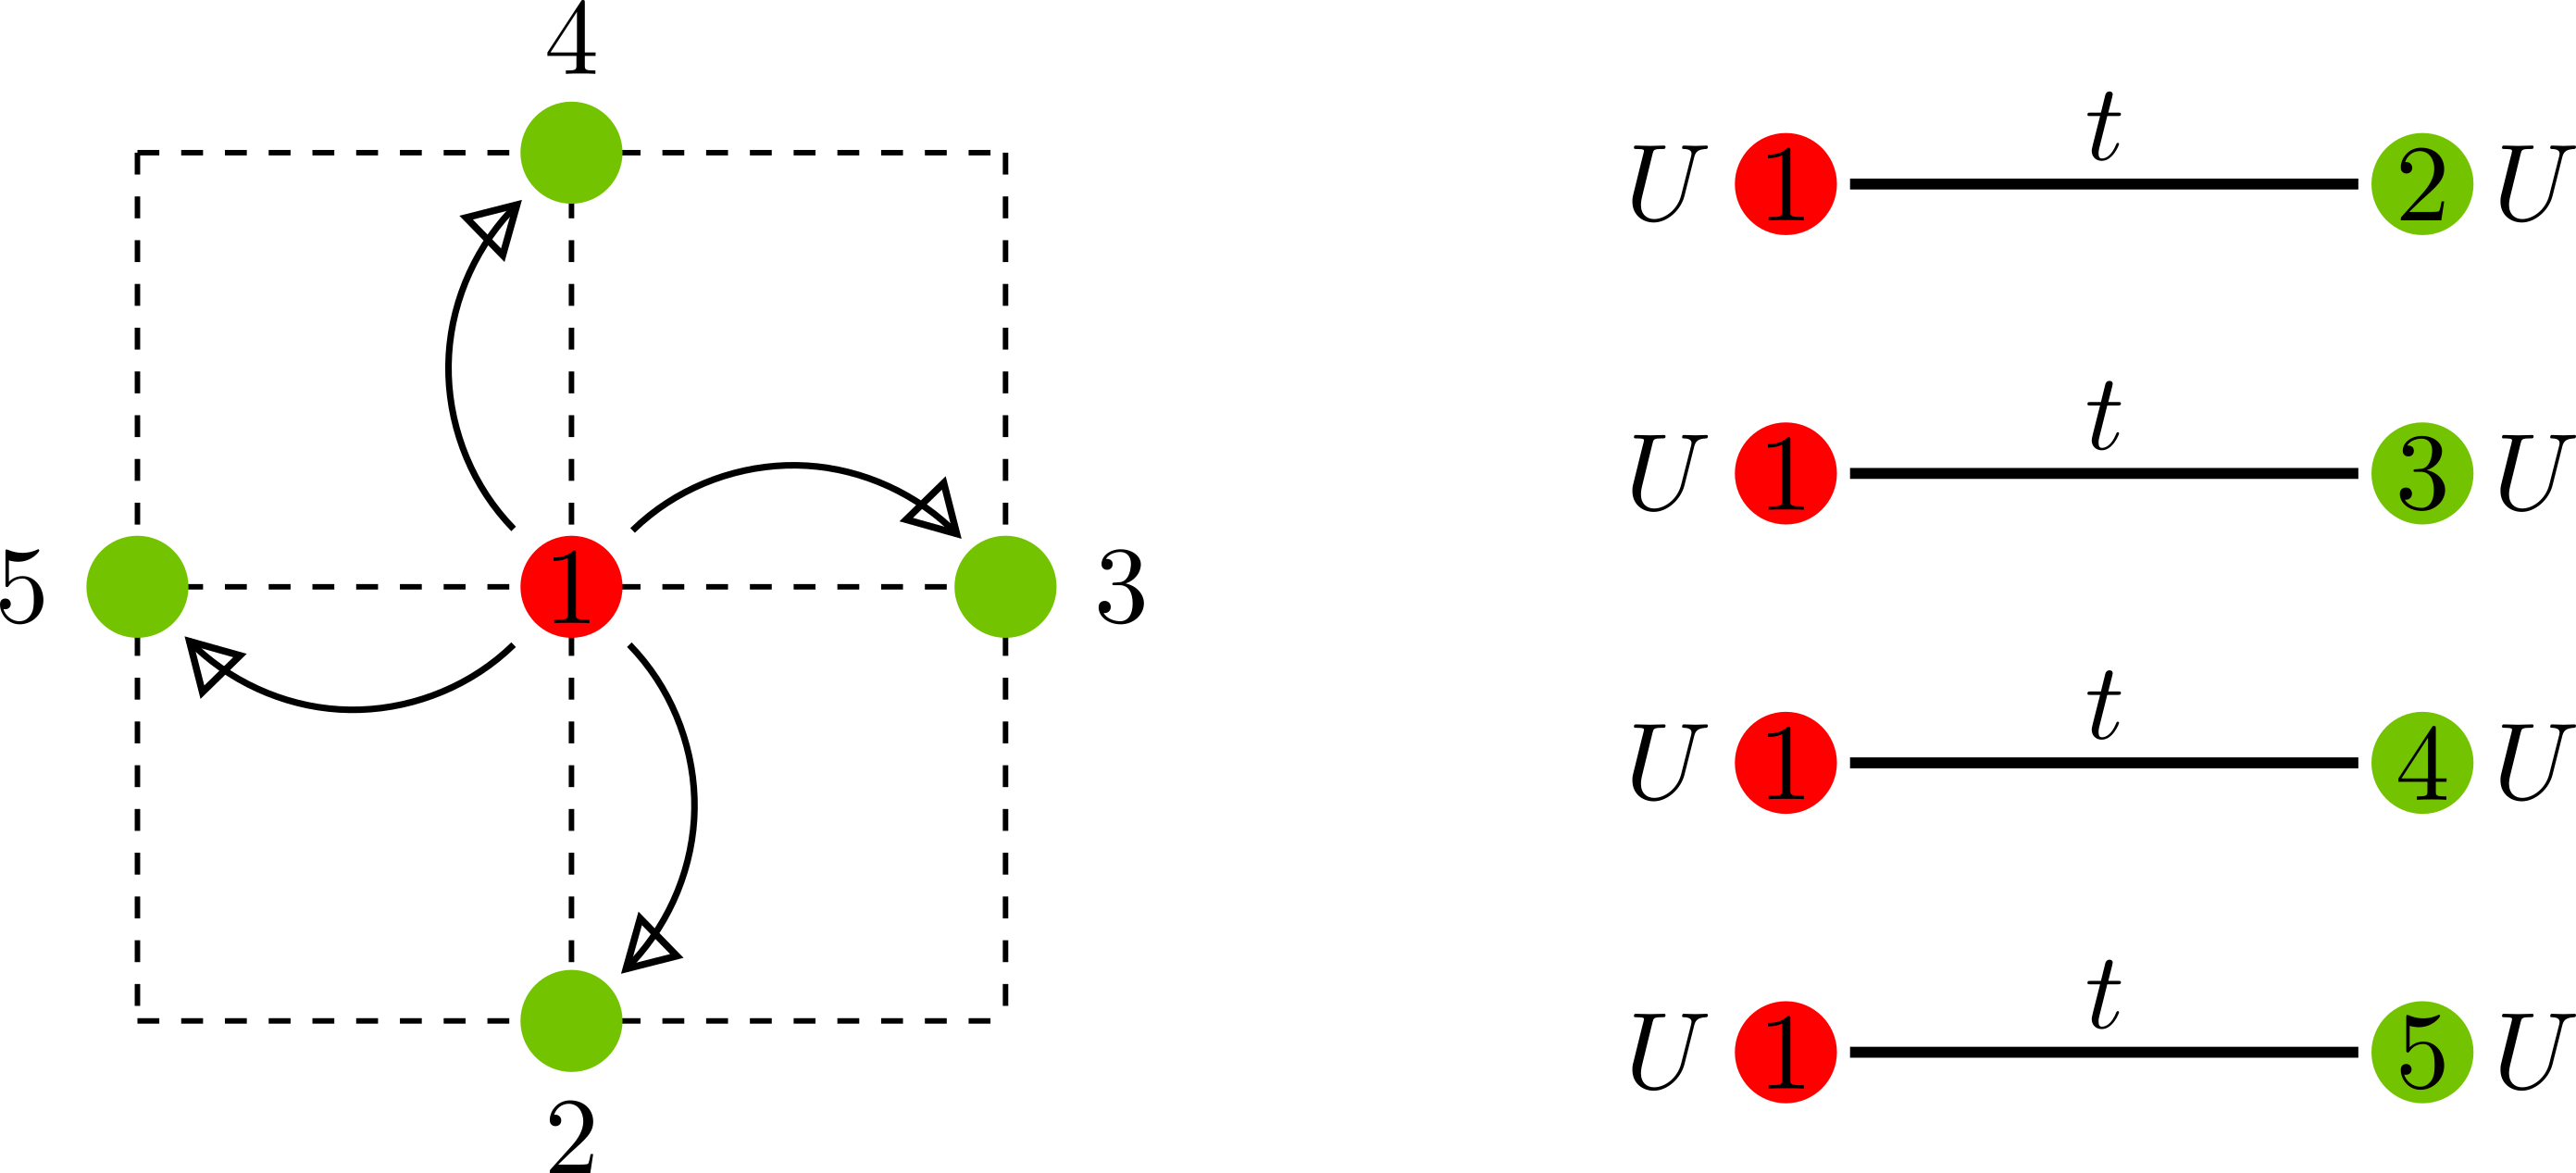
\includegraphics[width=0.7\textwidth]{./lattice.png}
	\hspace*{\fill}
	\caption{\textit{Left:} Part of the lattice that is picked out by the Greens function on the LHS of eq.~\ref{local_gf}. \textit{Right:} Hamiltonian whose Greens functions appear on the right hand side of same equation. The two submodels are identical.}
\end{figure}
\subsection{Constructing full Greens function matrix from the inverse matrix via Fourier transformation to \(k-\)space}
Since the only real-space interaction is that between the nearest neighbours, there are no further real space Greens functions, and the matrix $G^{-1}$ is tridiagonal in real space. Because of translational invariance, we know that $\left(G_H^{-1}\right)_{ii}$ and $\left(G_H^{-1}\right)_{ij}$ are independent of $i,j$. Furthermore, all expressions below are for a particular spin $\sigma$; from the spin rotational symmetry of the Hubbard Hamiltonian, the same expressions are obtained for the opposite spin.
\begin{equation}\begin{aligned}
	G^{-1}_H(\omega) = \begin{pmatrix} \left(G^{-1}\right)_{00} & \left(G^{-1}\right)_{01} & ... & ... & \left(G^{-1}\right)_{0N}\\
		\left(G^{-1}\right)_{10} & \left(G^{-1}\right)_{11} & \left(G^{-1}\right)_{12} & ... & ...\\
		... & \left(G^{-1}\right)_{21} & \left(G^{-1}\right)_{22} & \left(G^{-1}\right)_{23} & ... \\
		    &&.&&\\
		    &&.&&\\
		    &&.&&\\
\end{pmatrix} = \begin{pmatrix} g_0 & g_1 & ... & ... & g_1\\
		g_1 & g_0 & g_1 & ... & ...\\
		... & g_1 & g_0 & g_1 & ... \\
		    &&...&&\\
		    &&...&&\\
\end{pmatrix} 
\end{aligned}\end{equation}
It can be written in the operator form as
\begin{equation}\begin{aligned}
	G_H^{-1}(\omega) = g_0\sum_{i=1}^N\ket{i}\bra{i} + g_1\sum_{\left<i,j \right>}^N\left( \ket{i}\bra{j} + \text{h.c.}\right)
\end{aligned}\end{equation}
We can Fourier transform the real space basis kets $\ket{i} \equiv \ket{\vec r_i}$ into momentum space:
\begin{flalign*}
	\ket{i} &= \frac{1}{\sqrt N}\sum_{\vec k=\vec k_1}^{\vec k_N} e^{i \vec{k}\cdot\vec{r_i}}\ket{\vec k} \Leftrightarrow \ket{k} = \frac{1}{\sqrt N}\sum_{\vec i} e^{-i \vec{k}\cdot\vec{r_i}}\ket{\vec r_i} \\
	\sum_i \ket{i}\bra{i} &= \frac{1}{N}\sum_i \sum_{\vec k, \vec q} e^{i \left(\vec{k} - \vec q\right)\cdot\vec{r_i}}\ket{\vec k}\bra{\vec q} = \frac{1}{N}\sum_{\vec k, \vec q} N \delta\left(\vec{k} - \vec q\right)\ket{\vec k}\bra{\vec q} = \sum_{\vec k=\vec k_1}^{\vec k_N} \ket{\vec k}\bra{\vec k}\\
	\sum_{\left<i,j \right>} \ket{i}\bra{j} &= \frac{1}{N}\sum_{\left<i,j \right>} \sum_{\vec k, \vec q} e^{i \left(\vec{k}\cdot \vec r_i - \vec q\cdot \vec r_j\right)}\ket{\vec k}\bra{\vec q} = \frac{1}{N}\frac{1}{2}\sum_{\hat e_i = \hat e_1}^{\hat e_D}\sum_{\vec k, \vec q} e^{-i\vec q\cdot a_i\hat e_i}\ket{\vec k}\bra{\vec q}\sum_{i=1}^N e^{i \left(\vec{k} - \vec q\right)\cdot \vec r_i} & \left[\sum_{\left<i,j \right>} = \frac{1}{2}\sum_i \sum_{j \in \text{NN of i}}\right] \\
					&=\frac{1}{2}\sum_{\hat e_i = \hat e_1}^{\hat e_D}\sum_{\vec q} e^{-i\vec q\cdot \vec e_i}\ket{\vec q}\bra{\vec q} = \frac{1}{2}\sum_{\vec q} \left(\sum_{i_1}^{D}e^{-ia_iq_i}\right)\ket{\vec q}\bra{\vec q}
\end{flalign*}
$\hat e_i$ are the primitive lattice unit vectors for the general $d-$dimensional lattice. $q_i$ are the projections of $\vec q$ along those vectors. $a_i$ are the lattice spacings along each primitive vector. Adding the Hermitian conjugate simply extracts the real part:
\begin{equation}\begin{aligned}
	\sum_{\left<i,j \right>} \ket{i}\bra{j} + \text{h.c.} =\sum_{\vec q} \underbrace{\sum_{i_1}^{D}\cos\left(a_iq_i\right)}_{\equiv \xi_{\vec q}}\ket{\vec q}\bra{\vec q}
\end{aligned}\end{equation}
On a 2D square lattice, for instance, we obtain
\begin{eqnarray}
\xi_{\vec{q}} &=& 2(\cos q_{x}a_{x} + \cos q_{y}a_{y})\equiv \frac{-\epsilon_{\vec{q}}}{t^{H}}~,\nonumber\\
\epsilon_{\vec{q}} &=& -2t^{H}(\cos q_{x}a_{x} + \cos q_{y}a_{y})~.\label{2dsquaretb}
\end{eqnarray}
The inverse Greens function thus becomes diagonal in momentum space
\begin{equation}\begin{aligned}
G_H^{-1}(\omega) = \sum_{\vec k=\vec k_1}^{\vec k_N}\left(g_0 + g_1 \xi_{\vec k}\right)\ket{\vec k}\bra{\vec k} = \begin{pmatrix} g_0 + g_1\xi_{\vec k_1} &&& \\
	& g_0 + g_1\xi_{\vec k_2} && \\
	&& g_0 + g_1\xi_{\vec k_3} & \\
	...&...&...&\\
	\end{pmatrix} 
\end{aligned}\end{equation}
The matrix entries are written in momentum space, and the matrix is diagonal in this basis.
\subsection{Calculation of self energy matrix from the Dyson equation}
Using Dyson's equation for the self-energy $\Sigma = G_{0}^{-1} - G^{-1}$ (where the matrix $G_{0,H}^{-1} (\omega) = \sum_{\vec k=\vec k_1}^{\vec k_N} (\omega -\epsilon_{k})\ket{\vec k}\bra{\vec k}=\sum_{\vec k=\vec k_1}^{\vec k_N} (\omega +t^{H}\xi_{k})\ket{\vec k}\bra{\vec k} $ is the inverse Greens function for the appropriate non-interacting tight-binding system), we obtain the self-energy matrix as
\begin{eqnarray}
\Sigma_{H} (\omega) &=& G_{0,H}^{-1} - G_{H}^{-1}~,\nonumber\\
&=&\sum_{\vec k=\vec k_1}^{\vec k_N} (\omega - g_{0} + (t^{H} - g_{1})\xi_{\vec{k}})\ket{\vec k}\bra{\vec k}
\end{eqnarray}
This is the full self energy matrix. One can get both real space and momentum space self energies by taking appropriate matrix elements. For instance, the self-energy in momentum space is
\begin{equation}\begin{aligned}
	\label{selfenergy}
	\Sigma_{H} (\vec{k},\omega) \equiv \bra{\vec k} \Sigma_H (\omega) \ket{\vec k} = \omega - g_{0} + (t^{H} - g_{1})\xi_{\vec{k}}~.
\end{aligned}\end{equation}
Thus, we can use eqs.\eqref{2dsquaretb}, \eqref{local_gf} and \eqref{nn_gf} to obtain the full self-energy $\Sigma (\vec{k},\omega)$ for the Hubbard model on the 2D square lattice.
\subsection{Obtaining real space Greens functions from the full matrix}
Since $G_H^{-1}(\omega)$ is diagonal in this basis, we can invert the matrix trivially by replacing the diagonal elements with their reciprocals.
\begin{equation}\begin{aligned}
	\label{k-space-gf}
	G_H(\omega) = \sum_{\vec k=\vec k_1}^{\vec k_N}\left(g_0 + g_1 \xi_{\vec k}\right)^{-1}\ket{\vec k}\bra{\vec k} = \begin{pmatrix} \left(g_0 + g_1\xi_{\vec k_1}\right)^{-1} &&&&\\
	& \left(g_0 + g_1\xi_{\vec k_2}\right)^{-1} &&&\\
	&& \left(g_0 + g_1\xi_{\vec k_3}\right)^{-1} &&\\
		...&&&...&\\
	\end{pmatrix} 
\end{aligned}\end{equation}
The diagonal elements of $G_H$ in momentum space are simply $G_H(\vec k, \omega)$
\begin{equation}\begin{aligned}
	G_H(\vec k, \omega) &= \left(g_0 + g_1 \xi_{\vec k}\right)^{-1}\\
			    &= \left\{\frac{2}{N}\left[G_{D}^{-1}(\omega)\right]_{00\sigma} + \frac{2}{Nw}\left[G_{D}^{-1}(\omega)\right]_{01\sigma}\xi_{\vec k}\right\}^{-1}\\
			    &= \frac{N}{2}\left\{\left[G_{D}^{-1}(\omega)\right]_{00\sigma} + \frac{1}{w}\left[G_{D}^{-1}(\omega)\right]_{01\sigma}\xi_{\vec k}\right\}^{-1}\\
\end{aligned}\end{equation}
The real-space Greens functions can now be obtained by taking matrix elements of the full Greens function matrix in eq.~\ref{k-space-gf}:
\begin{equation}\begin{aligned}
	G_H(\vec r_i, \vec  r_j, \omega) \equiv \bra{\vec r_i} G_H(\omega) \ket{\vec r_j} = \sum_{\vec k} G_H(\vec k, \omega)  \left<\vec r_i | \vec k\right>\left<\vec k | \vec r_j\right>
\end{aligned}\end{equation}
From the definition of the Fourier transforms mentioned previously, we can write
\begin{equation}\begin{aligned}
	\left<\vec r_i | \vec k\right> = \frac{1}{\sqrt N}\sum_{\vec r} e^{- \vec{k}\cdot\vec{r}} \left<\vec r_i | \vec r \right> = \frac{1}{\sqrt N}e^{- \vec{k}\cdot\vec{r_i}}
\end{aligned}\end{equation}
Substituting this gives
\begin{equation}\begin{aligned}
	G_H(\vec r_i, \vec  r_j, \omega) = \frac{1}{N}\sum_{\vec k} G_H(\vec k, \omega)  e^{\vec{k}\cdot\left(\vec r_j - \vec{r_i}\right)} \equiv G_H(\vec r_j - \vec  r_i, \omega)
\end{aligned}\end{equation}
The final expression brings out the fact that the Greens function for excitations between \(\vec r_i\) and \(\vec r_j\) depends only on the relative position \(\vec r_j - \vec r_i\), not on their absolute positions. This is expected on grounds of translational invariance. By choosing \(\vec r_i = \vec r_j\), we can obtain the real space \textit{local} Greens function:
\begin{equation}\begin{aligned}
	\left(G_H\right)_{ii}(\omega) \equiv G_H(\vec r_j - \vec  r_i = 0, \omega) = \frac{1}{N}\sum_{\vec k} G_H(\vec k, \omega) = \frac{1}{N}\sum_{\vec k}\left(g_0 + g_1 \xi_{\vec k}\right)^{-1}
\end{aligned}\end{equation}
We can now compute the $k$-space spectral function $A_{H}(\vec{k},\omega)$ and the real-space local spectral function $A_{H}(\vec{r}=0,\omega)$ as
\begin{equation}\begin{aligned}
A_{H}(\vec{k},\omega) &= -\frac{1}{\pi} \textrm{Im}(G_{H}(\vec{k},\omega)) = -\frac{1}{\pi} \textrm{Im}\left[ (g_{0} + g_{1}\xi_{\vec{k}})^{-1}\right]\\
A_{H}(\vec{r}=0,\omega) &= -\frac{1}{\pi} \textrm{Im}(G_{H}(\vec{r}=0,\omega)) = -\frac{1}{N\pi} \textrm{Im}\left[\sum_{\vec{k}} (g_{0} + g_{1}\xi_{\vec{k}})^{-1}\right] = -\frac{1}{N}\sum_{\vec{k}}A_{H}(\vec{k},\omega)
\end{aligned}\end{equation}
We can again use eqs.\eqref{2dsquaretb}, \eqref{local_gf} and \eqref{nn_gf} to obtain the spectral functions  $A_{H} (\vec{k},\omega)$ and $A_{H} (\vec{r}=0,\omega)$ for the Hubbard model on the 2D square lattice.
\subsection{Obtaining \(g_0\) and \(g_1\)}
These two quantities are expressed in terms of matrix elements of the inverse Greens function \(G_D^{-1}\) of the Hubbard dimer. Since \(G_D\) is a \(2\times 2\) matrix, it is easy to invert:
\begin{equation}\begin{aligned}
	G_D &= \begin{pmatrix} \left(G_D\right)_{00} &  \left(G_D\right)_{01} \\ \left(G_D\right)_{01} & \left(G_D\right)_{00}\end{pmatrix} \\
	\implies G_D^{-1} &= \frac{1}{\text{Det }G_D}\begin{pmatrix} \left(G_D\right)_{00} &  -\left(G_D\right)_{01} \\ -\left(G_D\right)_{01} & \left(G_D\right)_{00}\end{pmatrix}\\
		 \implies g_0 &\equiv\frac{2}{N} (G^{-1}_{D})_{00} = \frac{2}{N} \frac{1}{\text{Det }G_D}\left(G_D\right)_{00},\\
		 g_1 &\equiv\frac{2}{Nw} (G^{-1}_{D})_{00} = -\frac{2}{Nw}\frac{1}{\text{Det }G_D}\left(G_D\right)_{01} 
\end{aligned}\end{equation}
Using the expressions for $(G_{D})_{00}$ and $(G_{D})_{01}$ shown in the appendix, we can obtain $g_{0}$ and $g_{1}$ very generally. 

\section{Analytic consistency checks}
\subsection{Single-particle Greens function and self energy for the Hubbard dimer}
The simplest test involves calculating \(G_H(\vec r = 0, \omega)\) for the Hubbard dimer \(\left(N = 2, w = 1 \right)\). The discrete set of momenta are \(\left\{ \vec k_n \right\} = 0, \frac{\pi}{a}\), so
\begin{equation}\begin{aligned}
	\left\{\xi_{\vec k}\right\} = 1, -1
\end{aligned}\end{equation}
Therefore, the Greens function at $\vec r=0$ for the Hubbard dimer can be expressed as
\begin{equation}\begin{aligned}
	G_H(\vec r = 0, \omega) = \frac{1}{2}\left[\frac{1}{g_0 + g_1} + \frac{1}{g_0 - g_1}\right]  = \frac{g_0}{g_0^2 - g_1^2}
\end{aligned}\end{equation}
For the Hubbard dimer, we substitute $N=2, w=1$ into the expressions for $g_{0}$ and $g_{1}$ to obtain
\begin{equation}\begin{aligned}
	&g_0 = \frac{1}{\text{Det }G_D}\left( G_D \right)_{00}, &g_1 = -\frac{1}{\text{Det }G_D}\left( G_D \right)_{01}
\end{aligned}\end{equation}
The Greens function at the zeroth site then becomes
\begin{equation}\begin{aligned}
	G_H(\vec r = 0, \omega) = \text{Det }G_D\frac{\left(G_D\right)_{00}}{\left(G_D\right)_{00}^2 - \left(G_D\right)_{01}^2} = \text{Det }G_D\frac{\left(G_D\right)_{00}}{\text{Det }G_D} = \left(G_D\right)_{00}
\end{aligned}\end{equation}
This is the expected result. Because the full Hubbard model in this case was simply the Hubbard dimer, \(G_H(\vec r = 0, \omega)\) should just be \(\left(G_D\right)_{00}\). Although this is a trivial example (we matched the Hubbard dimer with another Hubbard dimer), this atleast tells us that this algorithm for calculating the real space local Greens function from the inverse Greens function matrix elements is sensible.

\subsection{On the Bethe lattice}
Another test involves considering the case of infinite number of nearest neighbours $w\to\infty$ (the coordination number, and effectively the dimensionality). Here, as has been argued in the DMFT literature, the correct scaling of the $t^{H}$ hopping parameter is $t^{H}\to t^{H}/\sqrt{w}$ such that the kinetic energy of the associated tight-binding lattice model is finite. This allows for the competition between the kinetic and potential terms of the Hamiltonian to drive a metal-insulator transition in the limit of $w\to\infty$ as well. Further, it has been argued in the DMFT literature that the Greens function matrix of the Hubbard model on the Bethe lattice with $w\to\infty$ becomes purely local (i.e., it has vanishing inter-site matrix elements). We can also see this from eqs.\eqref{local_gf},\eqref{nn_gf} where $(G^{H})^{-1}$ matrix has no $k$ dependence as $(G^{H})^{-1}_{ij}\propto 1/w \to 0$ as $w\to\infty$. Thus, in the self-energy 
\begin{eqnarray}
\Sigma_{H} (\vec{k},\omega) &=& \omega - g_{0} + (t^{H} - g_{1})\xi_{\vec{k}}\nonumber\\
&\to & \lim_{w\to\infty} \omega - {g}_{0} + t^{H}\xi_{\vec{k}}~,
\end{eqnarray}
We can now see that even in the limit of $w\to\infty$, the competition between ${g}_{0}$ (the on-site repulsion) and the hopping related kinetic energy ($t^{H}\xi_{\vec{k}}$) can lead to a metal-insulator transition.
\par\noindent
While we have provided expressions for the single particle Greens functions of the $N$-site Hubbard model from their equivalent single particle Greens functions of the Hubbard dimer, we expect that eq.\eqref{green_eq_final} holds quite generally for the two-particle Greens function sector as well. We will provide these expressions at a later point in time. 
\newpage
\section*{Appendix: Spectra of Hubbard dimer and Anderson molecule}
%Here we document the spectra of the Hamiltonians in eqs.~\ref{hubb_dimer} and \ref{and_dimer}.
\begin{center}
	\begin{tabular}{|c|c|c|}
	\hline
	eigenstate & symbol & eigenvalue \\
	\hline
	$\ket{0,0}$ & $\ket{0}$ & \( \frac{U^H}{2}\)\\
	$ \frac{1}{\sqrt 2}\left(\ket{\sigma,0} \pm \ket{0,\sigma}\right)$ & $\ket{0\sigma_\pm}$ & \(\mp t^H\)\\
	$\ket{\sigma,\sigma}$ & $\ket{\sigma\sigma}$ & \( -\frac{U^H}{2}\)\\
	$ \frac{1}{\sqrt 2}\left(\ket{\uparrow,\downarrow} + \ket{\downarrow,\uparrow}\right)$ & $\ket{ST}$ & \( -\frac{U^H}{2}\)\\
	$ \frac{1}{\sqrt 2}\left(\ket{2,0} - \ket{0,2}\right)$ & $\ket{CS}$ & \( \frac{U^H}{2}\)\\
	$a_1(U^H, t^H) \frac{1}{\sqrt 2}\left(\ket{\uparrow,\downarrow} - \ket{\downarrow,\uparrow}\right) + a_2(U^H, t^H)\frac{1}{\sqrt 2}\left(\ket{2,0} + \ket{0,2}\right)$ & $\ket{-}$ & \(-\frac{1}{2}\Delta(U^H, t^H)\)\\
	$-a_2(U^H, t^H) \frac{1}{\sqrt 2}\left(\ket{\uparrow,\downarrow} - \ket{\downarrow,\uparrow}\right) + a_1(U^H, t^H)\frac{1}{\sqrt 2}\left(\ket{2,0} + \ket{0,2}\right)$ & $\ket{+}$ & \(\frac{1}{2}\Delta(U^H, t^H)\)\\
	$ \frac{1}{\sqrt 2}\left(\ket{\sigma,2} \pm \ket{2,\sigma}\right)$ & $\ket{2\sigma_\pm}$ & \(\pm t^H\)\\
	$\ket{2,2}$ & $\ket{4}$ & \( \frac{U^H}{2}\)\\
\hline
	\end{tabular}
	\captionof{table}{Spectrum of Hubbard dimer at half-filling}
	\label{hubb_dim_spectrum}
	\begin{tabular}{|c|c|c|}
	\hline
	eigenstate & symbol & eigenvalue\\
	\hline
	\(\ket{0,0}\) & \(\ket{0}\) & \(\frac{U^A}{4}\)\\
	\(a_1\left(U^A, t^A\right)\ket{\sigma,0} + a_2\left(U^A, t^A\right)\ket{0, \sigma}\) & \(\ket{0\sigma_-}\) & \(-\frac{1}{4}\Delta(U^A, t^A)\)\\
	\(-a_2\left(U^A, t^A\right)\ket{\sigma,0} + a_1\left(U^A, t^A\right)\ket{0, \sigma}\) & \(\ket{0\sigma_+}\) & \(\frac{1}{4}\Delta(U^A, t^A)\)\\
	\(\ket{\sigma,\sigma}\) & \(\ket{\sigma\sigma}\) & \(-\frac{U^A}{4}\)\\
	\(\frac{1}{\sqrt 2}\left(\ket{\uparrow, \downarrow} + \ket{\downarrow, \uparrow}\right)\) & \(\ket{ST}\) & \(-\frac{U^A}{4}\)\\
	\(\frac{1}{\sqrt 2}\left(\ket{2, 0} - \ket{0, 2}\right)\) & \(\ket{CS}\) & \(\frac{U^A}{4}\)\\
	$a_1( \frac{1}{2}U^A, t^A) \frac{1}{\sqrt 2}\left(\ket{\uparrow,\downarrow} - \ket{\downarrow,\uparrow}\right) + a_2( \frac{1}{2}U^A, t^A)\frac{1}{\sqrt 2}\left(\ket{2,0} + \ket{0,2}\right)$ & $\ket{-}$ & \(-\frac{1}{2}\Delta( \frac{1}{2}U^A, t^A)\)\\
	$-a_2(\frac{1}{2}U^A, t^A) \frac{1}{\sqrt 2}\left(\ket{\uparrow,\downarrow} - \ket{\downarrow,\uparrow}\right) + a_1(\frac{1}{2}U^A, t^A)\frac{1}{\sqrt 2}\left(\ket{2,0} + \ket{0,2}\right)$ & $\ket{+}$ & \(\frac{1}{2}\Delta(\frac{1}{2}U^A, t^A)\)\\
	\(a_1\left(U^A, t^A\right)\ket{\sigma,2} - a_2\left(U^A, t^A\right)\ket{2, \sigma}\) & \(\ket{2\sigma_-}\) & \(-\frac{1}{4}\Delta(U^A, t^A)\)\\
	\(a_2\left(U^A, t^A\right)\ket{\sigma,2} + a_1\left(U^A, t^A\right)\ket{2, \sigma}\) & \(\ket{2\sigma_+}\) & \(\frac{1}{4}\Delta(U^A, t^A)\)\\
	\(\ket{2,2}\) & \(\ket{4}\) & \(\frac{U^A}{4}\)\\
	\hline
	\end{tabular}
	\captionof{table}{Spectrum of Anderson molecule at particle-hole symmetry}
\end{center}
\section*{Appendix: Local Greens function for the Hubbard dimer}
From the spectral representation, we have the following expression for the local Greens function for the Hubbard dimer at site $0$:
\begin{equation}\begin{aligned}
	G_{D,00}^\sigma(\omega) = \frac{1}{Z}\sum_{m,n}||\bra{m}c_{i\sigma}\ket{n}||^2\left( e^{-\beta E_m} + e^{-\beta E_n}\right)\frac{1}{\omega + E_m - E_n}
\end{aligned}\end{equation}
$m,n$ sum over the exact eigenstates. $E_m, E_n$ are the corresponding energies. We are interested in teh $T \to 0$ Greens function. In that limit, all exponentials except that for the ground state $E_{gs}$ will die out. The exponential inside the summation will then cancel the exponential in the partition function.
\begin{equation}\begin{aligned}
	G_{D,00}^\sigma(\omega, T \to 0) &= \sum_{n}\left[||\bra{GS}c_{i\sigma}\ket{n}||^2\frac{1}{\omega + E_{GS} - E_n} + ||\bra{n}c_{i\sigma}\ket{GS}||^2\frac{1}{\omega + E_n - E_{GS}}\right]\\
					&= \sum_{n}\left[||\bra{n}c^\dagger_{i\sigma}\ket{GS}||^2\frac{1}{\omega + E_{GS} - E_n} + ||\bra{n}c_{i\sigma}\ket{GS}||^2\frac{1}{\omega + E_n - E_{GS}}\right]\\
\end{aligned}\end{equation}

The ground state $\ket{GS}$ is just the state $\ket{-}$ in the table \ref{hubb_dim_spectrum}. We will choose to look at $\sigma = \uparrow`$. Then,
\begin{equation}\begin{aligned}
	c_{1\uparrow}\ket{-} &= \frac{a_1}{\sqrt 2}\ket{0, \downarrow} + \frac{a_2}{\sqrt 2}\ket{\downarrow,0}\\
	c^\dagger_{1\uparrow}\ket{-} &= -\frac{a_1}{\sqrt 2}\ket{2, \uparrow} + \frac{a_2}{\sqrt 2}\ket{\uparrow,2}\\
\end{aligned}\end{equation}
The set of states $\ket{n}$ that give non-zero inner product $\ket{GS}$ are therefore
\begin{equation}\begin{aligned}
	\left\{ \ket{n} \right\} &= \ket{0\downarrow_\pm}\\
	||\bra{n}c_{\uparrow\sigma}\ket{GS}||^2 &= \frac{1}{4}\left(a_2 \pm a_1 \right)^2 = \frac{1}{4}\left(1 \pm 2a_1a_2\right)\\
	\left\{ E_n \right\} &= \mp t
\end{aligned}\end{equation}
for the second inner product, and
\begin{equation}\begin{aligned}
	\left\{\ket{n}\right\} &= \ket{2\uparrow_\pm}\\
	||\bra{n}c^\dagger_{\uparrow\sigma}\ket{GS}||^2 &= \frac{1}{4}\left( a_2 \mp a_1 \right)^2 = \frac{1}{4}\left(1 \mp 2a_1a_2\right)\\
	\left\{ E_n \right\} &= \pm t
\end{aligned}\end{equation}
for the first. The Greens function is therefore
\begin{equation}\begin{aligned}
	\label{dimer_local_G}
	G_{D,00}^\uparrow(\omega, T \to 0) &= \left( \frac{1}{2} + \frac{2t}{\Delta} \right) \frac{\omega}{\omega^2 - \left(\frac{\Delta}{2} - t\right) ^2} + \left( \frac{1}{2} - \frac{2t}{\Delta} \right) \frac{\omega}{\omega^2 - \left(\frac{\Delta}{2} + t\right) ^2} = G_{D,00}^\downarrow(\omega, T \to 0)~.
\end{aligned}\end{equation}
In the atomic limit $(t=0)$, the Greens function simplifies to
\begin{equation}\begin{aligned}
	G_{D,00}^\uparrow(\omega, T \to 0) \bigg\vert_\text{atomic} = \frac{\omega}{\omega^2 - \frac{1}{4}U^2}
\end{aligned}\end{equation}
In the atomic limit, the singly-occupied state has zero energy:
\begin{equation}\begin{aligned}
	E_1(t=0) = \bra{1,0}\left(U \tau_{0 \uparrow}\tau_{0 \downarrow} + U \tau_{1 \uparrow}\tau_{1 \downarrow}\right) \ket{1,0} = 0
\end{aligned}\end{equation}
We can write the atomic limit Greens function in terms of this energy and the self energy:
\begin{equation}\begin{aligned}
	G_{D,00}^\uparrow(\omega, T \to 0) \bigg\vert_\text{atomic} = \frac{1}{\omega - E_1(t=0) - \Sigma(t=0)} = \frac{1}{\omega - 0 -\frac{U^2}{4\omega}}
\end{aligned}\end{equation}
The self energy in the atomic limit can be read off as 
\begin{equation}\begin{aligned}
	\label{dimer_selfenergy}
\Sigma(t=0) = \frac{U^2}{4\omega}
\end{aligned}\end{equation}
The site local spectral function can also be calculated from the local Greens function:
\begin{eqnarray}
A(0\uparrow, \omega) &=& - \frac{1}{\pi}\text{Im }G_{D,00}^\uparrow(\omega)\nonumber\\
			     &=& \left( \frac{1}{4} - \frac{t}{\Delta} \right)\left[\delta(\omega - \frac{1}{2}\Delta - t) + \delta(\omega + \frac{1}{2}\Delta + t)\right]\nonumber\\ 
			     &&+ \left( \frac{1}{4} + \frac{t}{\Delta} \right) \left[\delta(\omega - \frac{1}{2}\Delta + t) + \delta(\omega + \frac{1}{2}\Delta - t)\right]\\ 
			     &=& A(0\downarrow, \omega)~.\nonumber
\end{eqnarray}
Finally, the inter-site Greens function for the Hubbard dimer is given by
\begin{equation}
\label{dimer_intersite_G}
	G_{D,01}^\uparrow(\omega, T \to 0) = \left( \frac{1}{2} + \frac{2t}{\Delta} \right) \frac{t}{(\omega +\frac{\Delta}{2})^2 - t^2} + \left( \frac{1}{2} - \frac{2t}{\Delta} \right) \frac{t}{(\omega -\frac{\Delta}{2})^2 - t^2} = G_{D,01}^\downarrow(\omega, T \to 0)~.
\end{equation}
%\section*{Appendix: Greens functions for Anderson molecule}
%\begin{equation}\begin{aligned}
%	G_{dd}^\uparrow(\omega) &= \sum_{n}\left[\frac{||\bra{n}c^\dagger_{d\uparrow}\ket{GS}||^2}{\omega + E_{GS} - E_n} + \frac{||\bra{n}c_{d\uparrow}\ket{GS}||^2}{\omega + E_n - E_{GS}}\right]\\
%	G_{zz}^\uparrow(\omega)&= \sum_{n}\left[\frac{||\bra{n}c^\dagger_{z\uparrow}\ket{GS}||^2}{\omega + E_{GS} - E_n} + \frac{||\bra{n}c_{z\uparrow}\ket{GS}||^2}{\omega + E_n - E_{GS}}\right]\\
%	G_{dz}^\uparrow(\omega)	&= \sum_{n}\left[\frac{\left<GS|c_{d\uparrow} | n \right>\left<n |c^\dagger_{z \uparrow} |GS\right>}{\omega + E_{GS} - E_n} + \frac{\left<n|c_{d\uparrow} | GS\right>\left<GS |c^\dagger_{z \uparrow} |n\right>}{\omega + E_{n} - E_{GS}}\right]\\
%	G_{zd}^\uparrow(\omega) &= \sum_{n}\left[\frac{\left<GS|c_{z \uparrow} | n \right>\left<n |c^\dagger_{d \uparrow} |GS\right>}{\omega + E_{GS} - E_n} + \frac{\left<n|c_{z \uparrow} | GS\right>\left<GS |c^\dagger_{d \uparrow} | n\right>}{\omega + E_{n} - E_{GS}}\right] = \left\{G_{dz}^\uparrow(\omega)\right\}^\dagger\\
%\end{aligned}\end{equation}
%We proceed exactly as before. With the following shorthand notations,
%\begin{equation}\begin{aligned}
%	a_{1,2} &\equiv a_{1,2}\left(U^A, t^A\right), &&\tilde a_{1,2} \equiv a_{1,2}\left(\frac{1}{2}U^A, t^A\right) \\
%	\Delta &\equiv \Delta\left(U^A, t^A\right), &&\tilde \Delta \equiv \Delta\left(\frac{1}{2}U^A, t^A\right)\\
%	C_z^\pm &\equiv a_1 \tilde a_1 \pm a_2 \tilde a_2, &&C_x^\pm \equiv a_1 \tilde a_2 \pm a_2 \tilde a_1
%\end{aligned}\end{equation}
%\begin{equation}\begin{aligned}
%	E_{\pm} \equiv E(\ket{2\sigma_\pm}) - E(\ket{-}) = E(\ket{0\sigma_\pm}) - E(\ket{-}) = \frac{1}{2}\tilde\Delta \pm \frac{1}{4}\Delta\\
%\end{aligned}\end{equation}
%the diagonal Green's functions are
%\begin{equation}\begin{aligned}
%	\label{mole_local_G}
%	G_{d d}^\uparrow(\omega) &= \left[a_1\tilde a_2 + a_2\tilde a_1\right]^2\frac{\omega}{\omega^2 - \left[\frac{1}{2}\tilde\Delta - \frac{1}{4}\Delta\right]^2 } +\left[a_1\tilde a_1 - a_2\tilde a_2\right]^2\frac{\omega}{\omega^2 - \left[\frac{1}{2}\tilde\Delta + \frac{1}{4}\Delta\right]^2 }\\
%				 &= {C_x^+}^2\frac{\omega}{\omega^2 - E_{-}^2 } +{C_z^-}^2\frac{\omega}{\omega^2 - E_{+}^2 }
%\end{aligned}\end{equation}
%\begin{equation}\begin{aligned}
%	G_{z z}^\uparrow(\omega) &= \left[a_1\tilde a_1 + a_2\tilde a_2\right]^2\frac{\omega}{\omega^2 - \left[\frac{1}{2}\tilde\Delta - \frac{1}{4}\Delta\right]^2 } +\left[a_1\tilde a_2 - a_2\tilde a_1\right]^2\frac{\omega}{\omega^2 - \left[\frac{1}{2}\tilde\Delta + \frac{1}{4}\Delta\right]^2 }\\
%				 &= {C_z^+}^2\frac{\omega}{\omega^2 - E_{-}^2 } +{C_x^-}^2\frac{\omega}{\omega^2 - E_{+}^2 }
%\end{aligned}\end{equation}
%and the off-diagonal Greens functions are
%\begin{equation}\begin{aligned}
%	G_{dz}^\uparrow(\omega) &= \left(a_1 \tilde a_1 + a_2 \tilde a_2\right) \left(a_1 \tilde a_2 + a_2 \tilde a_1\right) \frac{\frac{1}{4}\Delta - \frac{1}{2}\tilde\Delta}{\omega^2 - \left(\frac{1}{4}\Delta - \frac{1}{2}\tilde\Delta\right)^2} - \left(a_1 \tilde a_1 - a_2 \tilde a_2\right) \left(a_1 \tilde a_2 - a_2 \tilde a_1\right) \frac{\frac{1}{2}\tilde\Delta + \frac{1}{4}\Delta}{\omega^2  - \left(\frac{1}{2}\tilde\Delta + \frac{1}{4}\Delta\right)^2}\\
%				&= -C_z^+ C_x^+ \frac{E_{-}}{\omega^2 - E_{-}^2} - C_z^- C_x^- \frac{E_{+}}{\omega^2  - E_{+}^2}\\
%G_{zd}^\uparrow(\omega) &= {G_{dz}^\uparrow(\omega)}^\dagger = G_{dz}^\uparrow(\omega)
%\end{aligned}\end{equation}
%To summarize, the four Green's real space Greens functions, in the compact notation, of the Anderson molecule are
%\begin{equation}\begin{aligned}
%	G_{dd}^\uparrow(\omega) &= {C_x^+}^2\frac{\omega}{\omega^2 - E_{-}^2 } +{C_z^-}^2\frac{\omega}{\omega^2 - E_{+}^2 }\\
%	G_{zz}^\uparrow(\omega) &= {C_z^+}^2\frac{\omega}{\omega^2 - E_{-}^2 } +{C_x^-}^2\frac{\omega}{\omega^2 - E_{+}^2 }\\
%	G_{dz}^\uparrow(\omega) &= G_{zd}^\uparrow(\omega) = -C_z^+ C_x^+ \frac{E_{-}}{\omega^2 - E_{-}^2} - C_z^- C_x^- \frac{E_{+}}{\omega^2  - E_{+}^2}
%\end{aligned}\end{equation}

\bibliographystyle{unsrt}
\bibliography{notes}
\end{document}
